\documentclass[11pt,a4paper]{article}

\usepackage[utf8]{inputenc}
\usepackage[T1]{fontenc}
\usepackage{lmodern}
\usepackage[a4paper,top=1.8cm,bottom=1.8cm,left=2cm,right=2cm]{geometry}
\renewcommand{\familydefault}{\sfdefault}
\usepackage{setspace}
\onehalfspacing

\usepackage{amsmath,amssymb}
\usepackage{graphicx}
\usepackage{booktabs}
\usepackage{tabularx}
\usepackage{array}
\usepackage{multirow}
\usepackage{caption}
\usepackage{subcaption}
\usepackage{float}
\usepackage{url}
\urlstyle{same}
\usepackage[expansion=false]{microtype}
\usepackage[hidelinks]{hyperref}

% Breakable framed boxes matching official MUH401 format
\usepackage{framed}
\setlength{\FrameRule}{0.8pt}
\setlength{\FrameSep}{8pt}

% TOC formatting
\makeatletter
\renewcommand\tableofcontents{\@starttoc{toc}}
\renewcommand\listoftables{\@starttoc{lot}}
\renewcommand\listoffigures{\@starttoc{lof}}
\makeatother

\begin{document}

% ==============================================================================
% DOCUMENT HEADER
% ==============================================================================
\begin{center}
    {\Large \textbf{MUH401- INTERIM PROJECT REPORT FORMAT}}
\end{center}
\vspace{0.4em}

% ==============================================================================
% BOX 1: COVER PAGE
% ==============================================================================
\begin{framed}
\noindent\textbf{Cover Page}\\[0.4em]
\begin{center}
\renewcommand{\arraystretch}{1.25}
\begin{tabular}{r @{\hspace{0.8em}} l}
\textbf{Title of the Project:} & \parbox[t]{0.68\textwidth}{\raggedright \textbf{Machine Learning-Based Discrimination of Precipitation-Induced Radon Washout for Radiological Anomaly Detection in EPA RadNet Air Monitoring Network}} \\[0.8em]
\textbf{Course Name:} & MUH401 \\[0.4em]
\textbf{Department / Faculty:} & Department of Environmental Engineering / Faculty of Engineering \\[0.4em]
\textbf{University:} & Hacettepe University \\[0.4em]
\textbf{Student Name(s) \& ID(s):} & Necdet Ömer Barut (2230867059) \\[0.4em]
\textbf{Supervisor / Instructor:} & [Supervisor / Instructor Name] \\[0.4em]
\textbf{Submission Date:} & November 2026 \\[0.4em]
\textbf{Academic Year / Semester:} & 2026--2027 Fall Semester
\end{tabular}
\end{center}
\end{framed}

\vspace{0.6em}

% ==============================================================================
% BOX 2: ABSTRACT
% ==============================================================================
\begin{framed}
\noindent\textbf{ABSTRACT}\\[0.6em]
This interim report presents a physics-informed computational framework to address the widespread operational vulnerability of automated radiation monitoring networks caused by precipitation-induced radon progeny washout. During rainfall events, natural terrestrial radon daughters ($^{214}\text{Pb}$ and $^{214}\text{Bi}$) are scavenged from the atmosphere onto particulate air filters, generating sudden gross gamma count surges of +40\% to +180\% that closely mimic anthropogenic releases. Existing automated threshold systems trigger 53 to 83 false alarms per station-year in humid climates. This research develops a multi-modal machine learning discrimination framework that fuses 8-channel sodium iodide gamma spectrometry from the United States Environmental Protection Agency RadNet network with contemporaneous National Oceanic and Atmospheric Administration surface weather observations. The project evaluates 324,550 synchronous observation hours across five climatologically diverse stations spanning 2017 through 2025. Detection performance is benchmarked across 450 filter-synchronized synthetic release plumes covering industrial and reactor fission products ($^{137}\text{Cs}$, $^{131}\text{I}$, $^{134}\text{Cs}$, $^{60}\text{Co}$). Across a 20-seed evaluation, the physics-informed nuclear and weather-fused gradient boosted model (Feature Schema 3) reduces operational false alarms by 96.7\% down to 2.71 per station-year (and 2.63 at the 90\% target) while achieving 94.00\% detection. This project delivers an automated, field-deployable decision-support system eliminating meteorological false alarms in environmental radiation surveillance.\\[0.6em]
\noindent\textbf{Keywords:} Environmental Radiation Monitoring, EPA RadNet, Radon Washout, Gamma Spectrometry, Machine Learning, Anomaly Detection.
\end{framed}

\newpage

% ==============================================================================
% BOX 3: TABLE OF CONTENTS
% ==============================================================================
\begin{framed}
\noindent\textbf{TABLE OF CONTENTS}\\[0.6em]
\tableofcontents
\end{framed}

\vspace{0.6em}

% ==============================================================================
% BOX 4: LIST OF TABLES
% ==============================================================================
\begin{framed}
\noindent\textbf{LIST OF TABLES}\\[0.6em]
\listoftables
\end{framed}

\vspace{0.6em}

% ==============================================================================
% BOX 5: LIST OF FIGURES
% ==============================================================================
\begin{framed}
\noindent\textbf{LIST OF FIGURES}\\[0.6em]
\listoffigures
\end{framed}

\vspace{0.6em}

% ==============================================================================
% BOX 6: LIST OF ABBREVIATIONS
% ==============================================================================
\begin{framed}
\noindent\textbf{LIST OF ABBREVIATIONS}\\[0.6em]
\begin{tabular}{l l}
\textbf{API} & Application Programming Interface \\
\textbf{CPM} & Counts Per Minute \\
\textbf{eFDR} & Empirical False Discovery Rate \\
\textbf{EPA} & United States Environmental Protection Agency \\
\textbf{FA/yr} & False Alarms per Station-Year \\
\textbf{FWHM} & Full Width at Half Maximum \\
\textbf{GBDT} & Gradient Boosted Decision Tree (LightGBM) \\
\textbf{ISD} & Integrated Surface Dataset (NOAA) \\
\textbf{MLP} & Multi-Layer Perceptron \\
\textbf{NaI(Tl)} & Thallium-activated Sodium Iodide Scintillation Detector \\
\textbf{NCEI} & National Centers for Environmental Information \\
\textbf{NOAA} & National Oceanic and Atmospheric Administration \\
\textbf{NORM} & Naturally Occurring Radioactive Material \\
\textbf{OOD} & Out-of-Distribution \\
\textbf{ROC} & Receiver Operating Characteristic \\
\textbf{ROI} & Region of Interest \\
\textbf{UTC} & Coordinated Universal Time \\
\textbf{WMO} & World Meteorological Organization \\
\end{tabular}
\end{framed}

\newpage

% ==============================================================================
% BOX 7: 1. INTRODUCTION
% ==============================================================================
\begin{framed}
\refstepcounter{section}
\addcontentsline{toc}{section}{1. INTRODUCTION}
\noindent\textbf{1. INTRODUCTION}\\[0.6em]
\refstepcounter{subsection}
\addcontentsline{toc}{subsection}{1.1 Background of the Problem}
\noindent\textbf{1.1 Background of the Problem}\\[0.3em]
Continuous atmospheric radiation surveillance networks are operated worldwide by regulatory authorities to provide immediate detection of clandestine nuclear testing, industrial accidents, and radiological dispersion events. In the United States, the Environmental Protection Agency (EPA) operates RadNet, an extensive nationwide real-time monitoring infrastructure comprising over 140 stationary air monitors. Each monitoring unit continuously draws ambient air through a particulate filter and records gamma-ray emission rates using thallium-doped sodium iodide ($\text{NaI(Tl)}$) scintillation detectors. 

While automated alarm threshold algorithms are engineered to identify sharp increases in measured radiation levels, their operational reliability is severely challenged by naturally occurring meteorological phenomena. Atmospheric precipitation scavenges airborne daughter radionuclides of radon-222 ($^{222}\text{Rn}$), primarily lead-214 ($^{214}\text{Pb}$) and bismuth-214 ($^{214}\text{Bi}$), depositing them directly onto the ground surface and particulate filter media. This phenomenon, known as radon washout, causes gross gamma count rates to surge by $+40\%$ to $+180\%$ above the dry baseline within 1 to 3 hours, persisting for several hours before radioactive decay restores nominal background levels.

\vspace{0.6em}
\refstepcounter{subsection}
\addcontentsline{toc}{subsection}{1.2 Problem Statement}
\noindent\textbf{1.2 Problem Statement}\\[0.3em]
Conventional automated radiation monitoring networks rely on static or rolling baseline thresholds (e.g., $3\sigma$ or $5\sigma$ deviations above a 168-hour moving average). Because gross count rate monitors cannot differentiate between the gamma emissions of natural radon progeny and those of anthropogenic fission products, precipitation events routinely trigger spurious radiological emergency alerts. In humid and temperate climates, such as the southeastern United States, standard $3\sigma$ threshold algorithms produce between 53 and 83 false alarm episodes per station-year, with over 32\% of these false alarms occurring synchronously with rainfall events. 

Conversely, raising the alert threshold to conservative levels (such as $5\sigma$) suppresses false alarms but severely degrades detection capability, dropping release detection probability below 10\% for low-to-moderate activity plumes. There is currently an acute lack of computationally efficient, causally sound methods capable of suppressing precipitation-induced false alarms while preserving rapid, highly sensitive detection of genuine radiological releases in real-time continuous surveillance.

\vspace{0.6em}
\refstepcounter{subsection}
\addcontentsline{toc}{subsection}{1.3 Importance and Relevance of the Study}
\noindent\textbf{1.3 Importance and Relevance of the Study}\\[0.3em]
The operational vulnerability created by weather-induced false alarms has substantial technical, environmental, and societal ramifications:
\begin{itemize}
    \item \textbf{Operational Integrity and Alarm Fatigue:} Frequent false alarms desensitize emergency personnel, increasing the hazard that a genuine radiological incident may be dismissed as a weather-induced anomaly.
    \item \textbf{Public Safety and Societal Impact:} Premature public notification of false emergencies causes widespread public panic, costly evacuations, and disruption of municipal infrastructure.
    \item \textbf{Economic Efficiency:} Dispatching mobile radiological inspection teams to investigate recurring spurious anomalies incurs substantial governmental operational expenditures.
    \item \textbf{Scientific Contribution:} By integrating multi-channel scintillation spectrometry with multi-scale atmospheric thermodynamic features, this research establishes a foundational methodology for automated, physics-grounded environmental surveillance.
\end{itemize}

\vspace{0.6em}
\refstepcounter{subsection}
\addcontentsline{toc}{subsection}{1.4 Clear Aim and Objectives of the Project}
\noindent\textbf{1.4 Clear Aim and Objectives of the Project}\\[0.3em]
The primary aim of this project is to develop, validate, and benchmark an automated, physics-informed machine learning framework that discriminates precipitation-induced radon washout spikes from genuine anthropogenic radiological anomalies in near-real-time environmental surveillance networks. Specific technical objectives include:
\begin{enumerate}
    \item Harmonize and process longitudinal multi-channel gamma spectrometry from EPA RadNet and contemporaneous surface meteorology from the NOAA Integrated Surface Dataset (ISD) across five climatologically distinct monitoring stations spanning nine full calendar years (2017--2025).
    \item Engineer a strictly causal real-time feature space that captures differential gamma spectral peak ratios ($^{214}\text{Pb}$, $^{214}\text{Bi}$ vs. $^{137}\text{Cs}$, $^{131}\text{I}$, $^{60}\text{Co}$) and antecedent precipitation dynamics without future lookahead bias.
    \item Formulate a three-class gradient boosted decision tree (LightGBM) architecture to continuously categorize observations into dry background, radon washout, or anthropogenic release.
    \item Conduct a multi-seed benchmark against conventional statistical baselines and rain-masked control rules over 450 synthetic radiological releases to prove false alarm reduction at matched detection power.
\end{enumerate}

\vspace{0.6em}
\refstepcounter{subsection}
\addcontentsline{toc}{subsection}{1.5 Scope and Boundaries of the Study}
\noindent\textbf{1.5 Scope and Boundaries of the Study}\\[0.3em]
The scope of this project encompasses five EPA RadNet monitoring stations selected across distinct Köppen climate zones: Birmingham, AL (humid subtropical, primary testbed); Little Rock, AR; Boise, ID (semi-arid); Concord, NH (humid continental); and Honolulu, HI (tropical). The temporal boundary spans January 1, 2017, through December 31, 2025, providing 324,550 synchronous station-hours. 

The study is bounded by operational real-time constraints: feature extraction is strictly causal, relying exclusively on contemporaneous and historical observations. Sensor inputs are restricted to standard 8-channel $\text{NaI(Tl)}$ energy bins ($100 - 2200\text{ keV}$) and standard NOAA meteorological observations. Source releases are evaluated through 450 synthetic plume injections calibrated to historical atmospheric dispersion physics, covering $^{137}\text{Cs}$, $^{131}\text{I}$, $^{134}\text{Cs}$, and $^{60}\text{Co}$.
\end{framed}

\newpage

% ==============================================================================
% BOX 8: 2. THEORETICAL BACKGROUND / LITERATURE REVIEW
% ==============================================================================
\begin{framed}
\refstepcounter{section}
\addcontentsline{toc}{section}{2. THEORETICAL BACKGROUND / LITERATURE REVIEW}
\noindent\textbf{2. THEORETICAL BACKGROUND / LITERATURE REVIEW}\\[0.6em]
\refstepcounter{subsection}
\addcontentsline{toc}{subsection}{2.1 Key Theories, Models, Concepts, and Definitions}
\noindent\textbf{2.1 Key Theories, Models, Concepts, and Definitions}\\[0.3em]
Radon-222 is an inert, noble gas daughter of radium-226 ($^{226}\text{Ra}$) in the primordial uranium-238 ($^{238}\text{U}$) decay series. Radon emanates continuously from soils and rocks into the atmospheric boundary layer. Because radon is chemically inert and has a half-life of 3.82 days, it diffuses into the lower troposphere, where it undergoes alpha decay into a sequence of short-lived particulate progeny:
\begin{equation}
    ^{222}\text{Rn} \xrightarrow[\alpha]{3.82\text{ d}} {}^{218}\text{Po} \xrightarrow[\alpha]{3.10\text{ m}} {}^{214}\text{Pb} \xrightarrow[\beta^-]{26.8\text{ m}} {}^{214}\text{Bi} \xrightarrow[\beta^-]{19.9\text{ m}} {}^{214}\text{Po} \xrightarrow[\alpha]{164.3\ \mu\text{s}} {}^{210}\text{Pb}
\end{equation}

Lead-214 ($^{214}\text{Pb}$) and bismuth-214 ($^{214}\text{Bi}$) rapidly attach to submicron ambient aerosol particles ($0.1 - 1.0\ \mu\text{m}$). During rainfall events, these radioactive aerosols are captured via in-cloud rainout (condensation nucleation) and below-cloud washout (impaction and interception by falling raindrops). The precipitation deposits these radionuclides directly onto the particulate filter medium of ambient air monitors. 

Because $^{214}\text{Pb}$ emits prominent gamma lines at $295.2\text{ keV}$ (18.4\% yield) and $351.9\text{ keV}$ (35.6\% yield), and $^{214}\text{Bi}$ emits high-energy gammas at $609.3\text{ keV}$ (45.5\%), $1120.3\text{ keV}$ (14.9\%), and $1764.5\text{ keV}$ (15.3\%), their sudden accumulation elevates the local gamma radiation field by tens to hundreds of counts per minute (CPM). Following the cessation of rain, the activity decay curve of the deposited progeny is governed by the effective half-life of the $^{214}\text{Pb}/^{214}\text{Bi}$ pair ($\sim 30 - 50\text{ minutes}$), returning to nominal baseline within 2 to 4 hours.

\vspace{0.6em}
\refstepcounter{subsection}
\addcontentsline{toc}{subsection}{2.2 Relevant Technical Background: Scintillation Spectrometry}
\noindent\textbf{2.2 Relevant Technical Background: Scintillation Spectrometry}\\[0.3em]
EPA RadNet deployable monitoring stations utilize thallium-activated sodium iodide ($\text{NaI(Tl)}$) scintillation crystals. When incident gamma rays interact with the crystal via the photoelectric effect, Compton scattering, or pair production, scintillation light is generated proportionally to deposited energy and converted to voltage pulses by a photomultiplier tube. While $\text{NaI(Tl)}$ detectors exhibit modest energy resolution ($\sim 7\%$ FWHM at $662\text{ keV}$), they are rugged, thermally stable, and well-suited for long-term field deployment.

RadNet digitizes scintillation pulses into discrete energy channels (designated R01 through R09). Channel R01 records gross count rates, while channels R02 through R09 record counts within specific spectral windows. The physical correspondence of these channels to natural radon progeny lines and target anthropogenic isotopes is detailed in Table~\ref{tab:energy_channels}.

\begin{center}
\captionof{table}{EPA RadNet Discrete Gamma Energy Channel Energy Boundaries}
\label{tab:energy_channels}
\small
\begin{tabularx}{\textwidth}{l c X X}
\toprule
\textbf{Channel} & \textbf{Energy Range (keV)} & \textbf{Principal Radon Progeny Lines} & \textbf{Target Anthropogenic Lines} \\
\midrule
\textbf{R02} & $101 - 200$ & Compton continuum & Low-energy scatter \\
\textbf{R03} & $201 - 400$ & $^{214}\text{Pb}$ ($295.2, 351.9\text{ keV}$) & $^{131}\text{I}$ ($364.5\text{ keV}$) \\
\textbf{R04} & $401 - 600$ & Compton continuum & Annihilation ($511\text{ keV}$) \\
\textbf{R05} & $601 - 800$ & $^{214}\text{Bi}$ ($609.3\text{ keV}$) & $^{137}\text{Cs}$ ($661.7\text{ keV}$) \\
\textbf{R06} & $801 - 1000$ & Compton scatter & Multi-line cascade \\
\textbf{R07} & $1001 - 1400$ & $^{214}\text{Bi}$ ($1120.3\text{ keV}$) & $^{60}\text{Co}$ ($1173.2, 1332.5$), $^{134}\text{Cs}$ \\
\textbf{R08} & $1401 - 1800$ & $^{214}\text{Bi}$ ($1764.5$), $^{40}\text{K}$ ($1460.8$) & Terrestrial background \\
\textbf{R09} & $1801 - 2200$ & High-energy background & Cosmic rays / actinide daughters \\
\bottomrule
\end{tabularx}
\end{center}

\vspace{0.6em}
\refstepcounter{subsection}
\addcontentsline{toc}{subsection}{2.3 Review of Relevant Previous Studies}
\noindent\textbf{2.3 Review of Relevant Previous Studies}\\[0.3em]
The challenge of suppressing meteorological radon interference in environmental monitoring networks has been addressed through three primary research paradigms:
\begin{enumerate}
    \item \textbf{Statistical Moving-Average Baselines:} Classical networks evaluate gross count deviations against moving baselines (Vieira et al., 2019). While computationally trivial, these methods are intrinsically blind to spectral morphology and trigger excessive false alarms during convective precipitation.
    \item \textbf{Analytical Meteorological Transfer Functions:} Huang et al. (2020) demonstrated that radon washout spikes correlate with precipitation intensity and cloud condensation lifting condensation levels. However, deterministic washout equations require high-resolution atmospheric sounding data rarely available at ground sensor sites.
    \item \textbf{Spectral Energy Ratio Heuristics:} Das et al. (2021) examined spectral ratios to differentiate radon progeny from industrial gamma sources, demonstrating that $^{214}\text{Pb}$ photopeaks in channel R03 exhibit distinct intensity ratios relative to channel R05 during washout events.
\end{enumerate}

\vspace{0.6em}
\refstepcounter{subsection}
\addcontentsline{toc}{subsection}{2.4 Gaps in Literature and Systematic Comparison}
\noindent\textbf{2.4 Gaps in Literature and Systematic Comparison}\\[0.3em]
Existing literature exhibits three critical shortcomings: (1) \textit{Gross count over-simplification:} Most operational networks discard multi-channel spectrometry and evaluate only total counts; (2) \textit{Synthetic release validation deficits:} Previous machine learning models were tested on uncalibrated synthetic data without accounting for air filter accumulation physics; and (3) \textit{Lack of honest control baselines:} Prior studies rarely compare complex models against simple meteorological masking rules. This project overcomes these gaps by fusing multi-channel spectral ratios with multi-scale weather data and benchmarking against both statistical and rain-masked baselines under frozen validation thresholds.
\end{framed}

\newpage

% ==============================================================================
% BOX 9: 3. METHODOLOGY
% ==============================================================================
\begin{framed}
\refstepcounter{section}
\addcontentsline{toc}{section}{3. METHODOLOGY}
\noindent\textbf{3. METHODOLOGY}\\[0.6em]
\refstepcounter{subsection}
\addcontentsline{toc}{subsection}{3.1 System Description and Processing Pipeline}
\noindent\textbf{3.1 System Description and Processing Pipeline}\\[0.3em]
The end-to-end computational pipeline developed in this project is illustrated in Figure~\ref{fig:architecture}. The framework ingests synchronous hourly observations from radiation and meteorological sensor networks, performs causal feature engineering, and feeds a gradient boosted decision tree classifier that assigns probabilities for three operational regimes: \textit{Clean Dry Background}, \textit{Radon Washout Anomaly}, and \textit{Anthropogenic Radiological Release}.

\begin{center}
    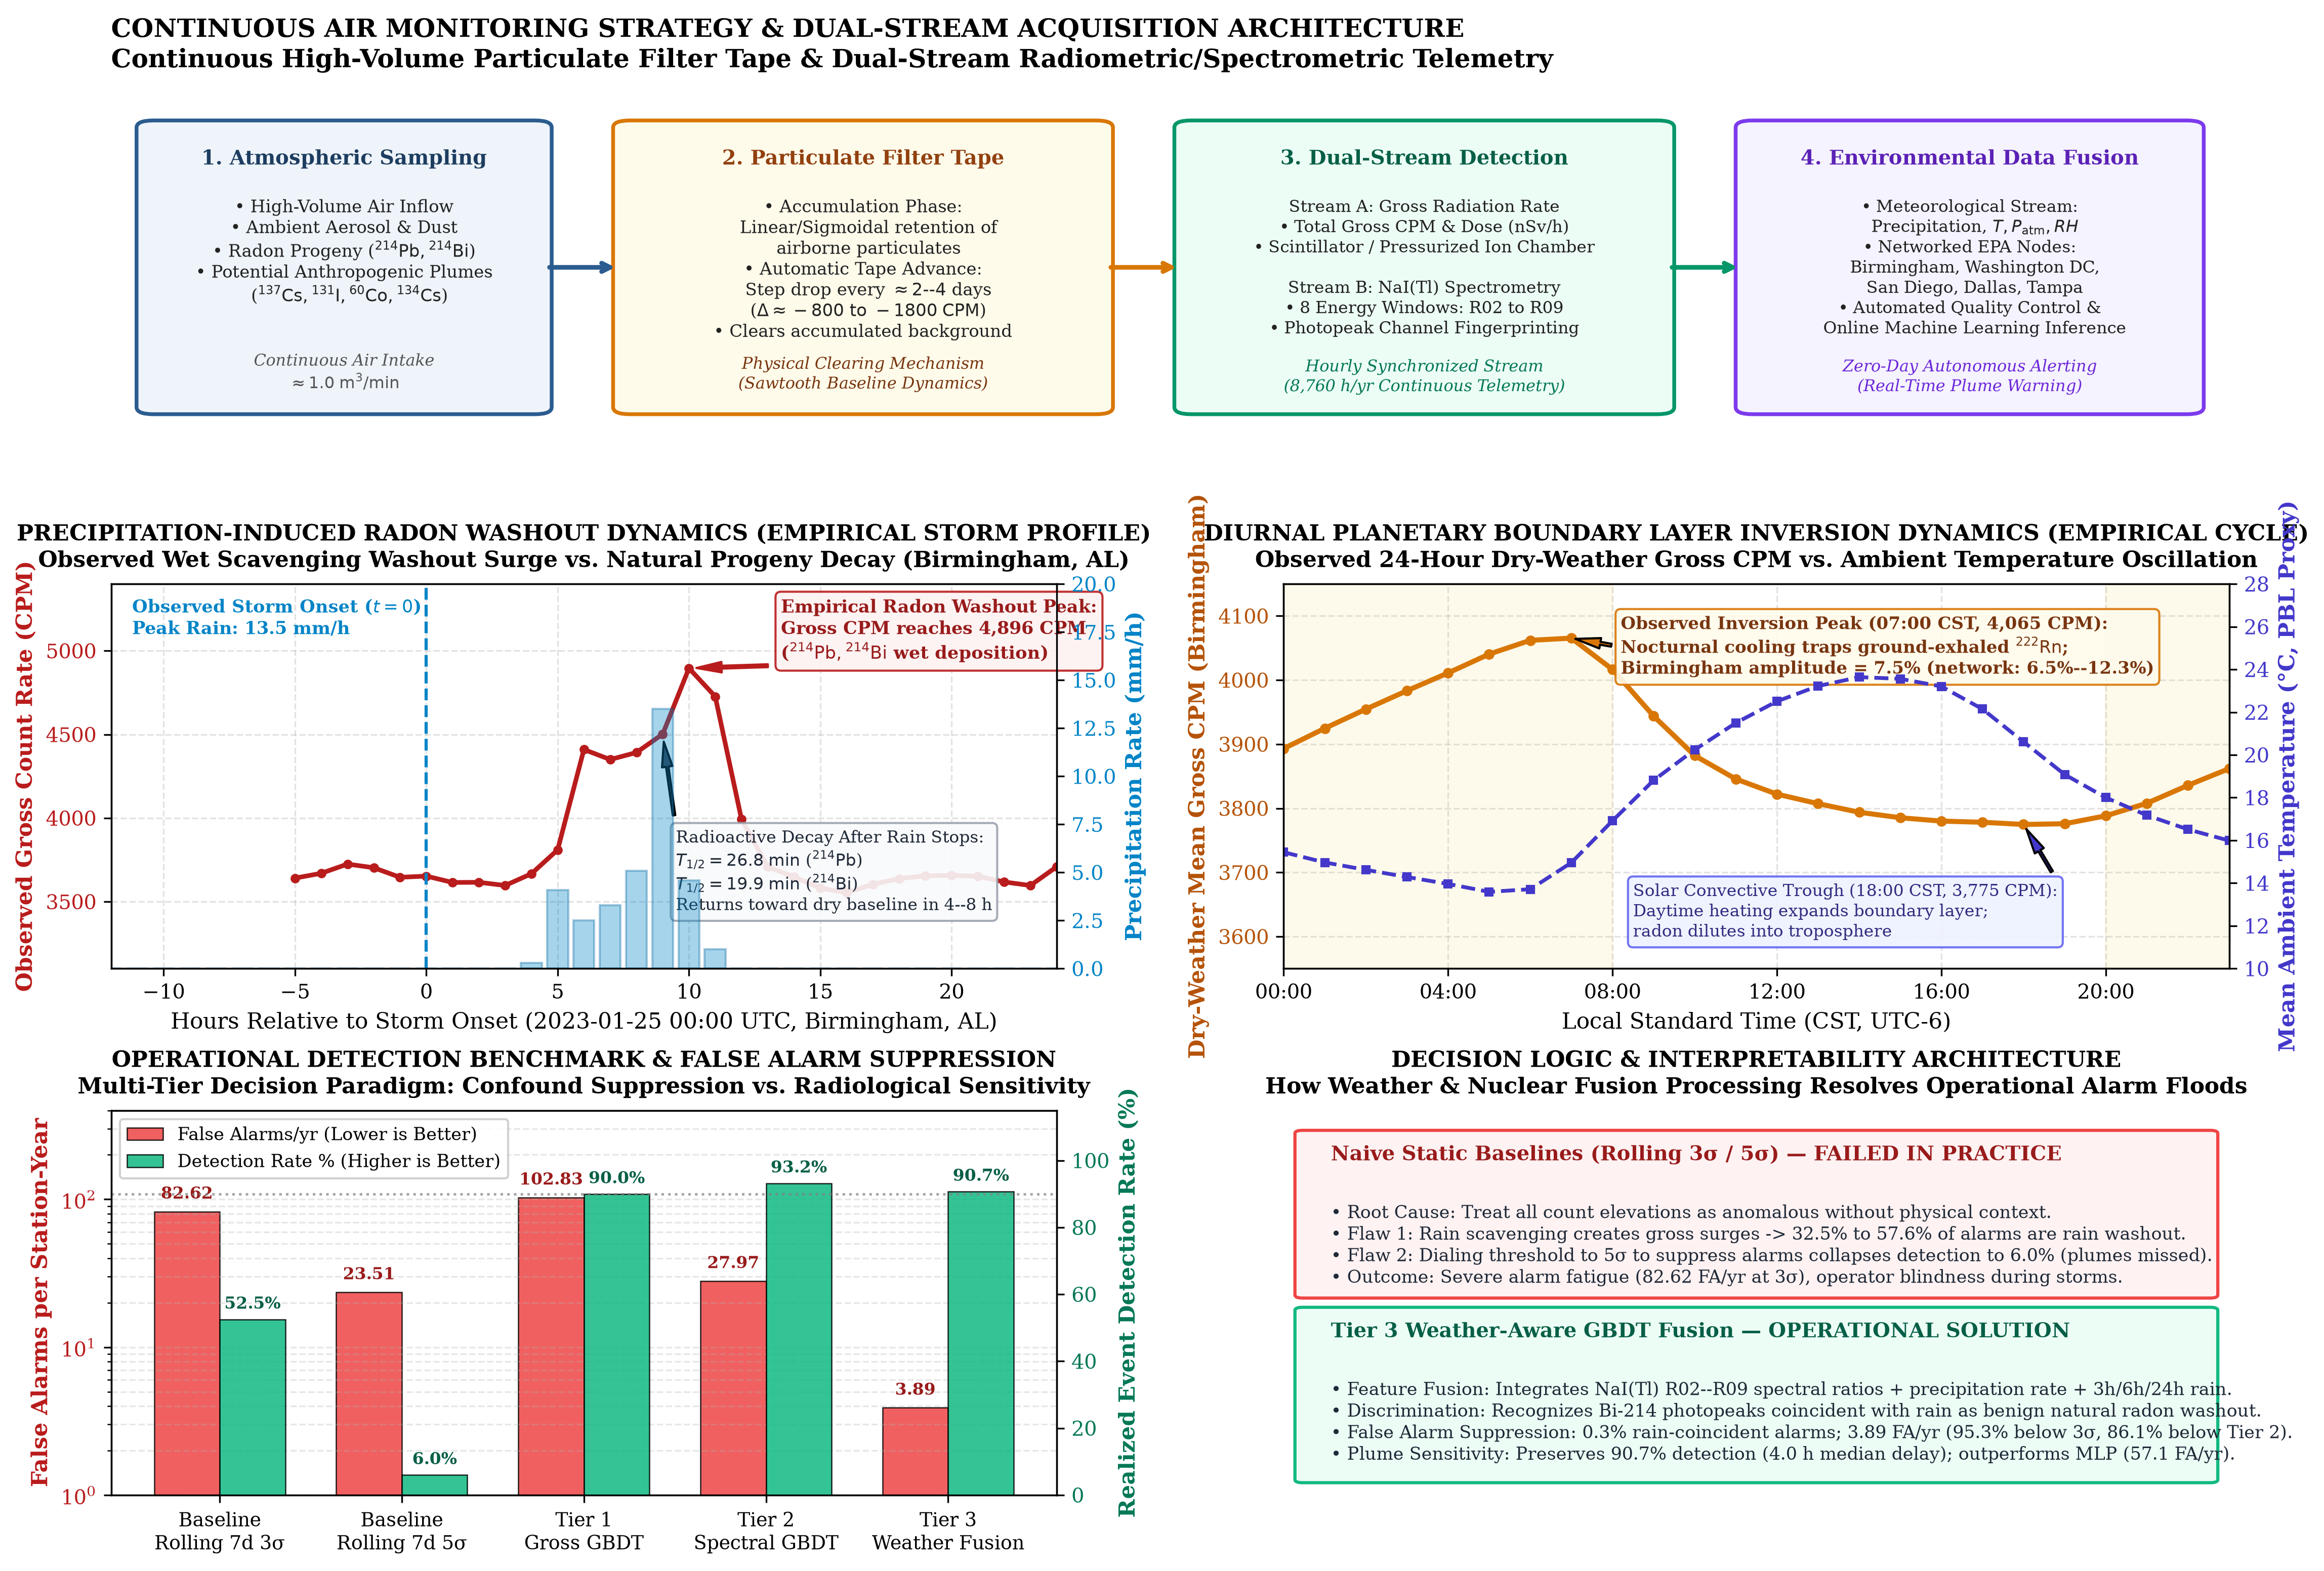
\includegraphics[width=0.86\textwidth]{reports/figures/environmental_engineering_synthesis.png}
    \captionof{figure}{End-to-end physics-informed environmental radiation anomaly detection and weather-fusion machine learning architecture.}
    \label{fig:architecture}
\end{center}

\vspace{0.6em}
\refstepcounter{subsection}
\addcontentsline{toc}{subsection}{3.2 Main Assumptions and Operational Boundaries}
\noindent\textbf{3.2 Main Assumptions and Operational Boundaries}\\[0.3em]
The computational architecture adheres to four rigorous operational boundaries:
\begin{enumerate}
    \item \textbf{Strict Real-Time Causality:} To prevent data leakage, all rolling window statistics (e.g., 24h, 168h means) are computed using closed-left intervals ($[t-W, t]$). No centered or forward-looking filters are permitted.
    \item \textbf{Air Filter Accumulation Dynamics:} Airborne particulate monitors draw air through a filter that is replaced periodically (nominally bi-weekly). An injection plume accumulates activity proportionally to total volume drawn, attenuating according to radioactive decay:
    \begin{equation}
        A_{\text{filter}}(t) = \int_{t_{\text{start}}}^t Q \cdot C_{\text{air}}(\tau) \cdot e^{-\lambda(t-\tau)} \, d\tau
    \end{equation}
    where $Q$ is volumetric flow rate ($\sim 1.0\text{ m}^3/\text{min}$), $C_{\text{air}}$ is ambient radionuclide concentration, and $\lambda$ is decay constant.
    \item \textbf{Detector Geometry and Efficiencies:} Geometric photopeak efficiencies for $\text{NaI(Tl)}$ crystals are calibrated using standard MCNP Monte Carlo transfer factors from Knoll (2010).
\end{enumerate}

\vspace{0.6em}
\refstepcounter{subsection}
\addcontentsline{toc}{subsection}{3.3 Input Data and Data Sources}
\noindent\textbf{3.3 Input Data and Data Sources}\\[0.3em]
Data ingestion leverages two primary US federal repositories:
\begin{itemize}
    \item \textbf{EPA RadNet Air Monitoring Network:} Hourly gamma spectrometry records across 8 discrete energy bins ($100 - 2200\text{ keV}$) and total gross count rates. Data were retrieved via EPA public APIs and FTP archives spanning 2017 through 2025 across five stations: Birmingham, AL; Little Rock, AR; Boise, ID; Concord, NH; and Honolulu, HI.
    \item \textbf{NOAA Integrated Surface Dataset (ISD):} Contemporaneous hourly meteorological observations from colocated automated surface observing stations (ASOS) at municipal airports. Variables include precipitation accumulation ($1\text{h}$, $3\text{h}$, $6\text{h}$), dry-bulb temperature, dew point, relative humidity, barometric pressure, wind speed, and present weather codes.
\end{itemize}

\vspace{0.6em}
\refstepcounter{subsection}
\addcontentsline{toc}{subsection}{3.4 Calculation Procedure and Causal Feature Engineering}
\noindent\textbf{3.4 Calculation Procedure and Causal Feature Engineering}\\[0.3em]
Radiological and meteorological records are joined on UTC timestamp rounded to the hour. The causal feature engineering engine extracts 28 dimensional variables organized into three tiers:
\begin{enumerate}
    \item \textbf{Gross Count Dynamics (Tier 1):} Ratio of instantaneous count rate to trailing 168-hour moving baseline ($R_{\text{gross}} = C(t) / \mu_{168\text{h}}$), rolling 3-hour rate of change ($dC/dt$), and z-score relative to local dry background ($\sigma_{\text{dry}}$).
    \item \textbf{Spectral Energy Ratios (Tier 2):} Normalized channel ratios capturing radon decay lines vs. fission product channels. Specifically:
    \begin{equation}
        \text{Ratio}_{\text{radon}} = \frac{R03 + R05}{R01 + \epsilon}, \quad \text{Ratio}_{\text{fission}} = \frac{R04 + R06 + R07}{R01 + \epsilon}
    \end{equation}
    Lead-214 ($352\text{ keV}$) concentrates heavily in R03, while bismuth-214 ($609\text{ keV}$) concentrates in R05. Anthropogenic releases ($^{137}\text{Cs}$ at $662\text{ keV}$, $^{134}\text{Cs}$ at $605, 796\text{ keV}$, $^{60}\text{Co}$ at $1173, 1332\text{ keV}$) alter these ratios markedly.
    \item \textbf{Multi-Scale Weather Fusion (Tier 3):} Cumulative precipitation over 1, 3, 6, 12, and 24 hours, hours elapsed since last detected rainfall ($h_{\text{since\_rain}}$), barometric pressure change ($dP/dt$), and saturation vapor pressure deficit calculated from temperature and dew point.
\end{enumerate}

\vspace{0.6em}
\refstepcounter{subsection}
\addcontentsline{toc}{subsection}{3.5 Synthetic Release Injections: 450 Plumes}
\noindent\textbf{3.5 Synthetic Release Injections: 450 Plumes}\\[0.3em]
Because real environmental data contains natural radon washout but fortunately zero lethal nuclear releases, genuine detection performance must be evaluated using synthetic injections. A library of 450 synthetic radiological plumes was generated across four target isotopes ($^{137}\text{Cs}$, $^{131}\text{I}$, $^{134}\text{Cs}$, $^{60}\text{Co}$) and three profile types (Gaussian puff, square wave, and asymmetric exponentially decaying plume with duration 3 to 24 hours). 

Synthetic plumes are scaled to signal-to-noise ratios ($\text{SNR} = \Delta C / \sigma_{\text{dry}}$) ranging from subtle ($0.5\sigma$ to $1.5\sigma$) to prominent ($2.0\sigma$ to $6.0\sigma$). Spectral counts are allocated across channels R02--R09 using calibrated photopeak and Compton continuum fractions, and added directly to real RadNet background series during both dry and rain-washout periods.

\vspace{0.6em}
\refstepcounter{subsection}
\addcontentsline{toc}{subsection}{3.6 Multi-Tier Model Formulation and Validation Freezing}
\noindent\textbf{3.6 Multi-Tier Model Formulation and Validation Freezing}\\[0.3em]
The machine learning framework utilizes LightGBM gradient boosted decision trees (Ke et al., 2017) configured with multi-class objective (\textit{multiclass}, 3 classes). Hyperparameters: 150 trees, max depth 6, learning rate 0.05, min child samples 20, colsample 0.8. 

\textit{Strict Validation Threshold Freezing:} Models are trained on historical data (2017--2021). The decision threshold $\tau$ for triggering an alert is calibrated on the validation split (2022) to satisfy a target detection probability (e.g., 90\% or 95\%) and frozen. The model and frozen threshold are evaluated strictly on the out-of-sample test split (2023--2025).

\vspace{0.6em}
\refstepcounter{subsection}
\addcontentsline{toc}{subsection}{3.7 Benchmark Evaluation across 20 Random Seeds}
\noindent\textbf{3.7 Benchmark Evaluation across 20 Random Seeds}\\[0.3em]
A 20-seed multi-model benchmark evaluation (seeds 42 to 61) was executed on the 2023--2025 test dataset. Performance metrics are summarized in Table~\ref{tab:benchmark_results}.

\begin{center}
\captionof{table}{Benchmark Evaluation on 2023--2025 Test Split across 20 Random Seeds}
\label{tab:benchmark_results}
\small
\resizebox{\textwidth}{!}{%
\begin{tabular}{l c c c c}
\toprule
\textbf{Model / Rule Architecture} & \textbf{False Alarms / Stn-Yr} & \textbf{Rain-Coincident FA} & \textbf{Realized Det. (\%)} & \textbf{Delay (h)} \\
\midrule
\textbf{Standard Baseline ($3\sigma_{168\text{h}}$)} & 82.62 & 32.5\% & 52.50\% & 10.0 \\
\textbf{Global Dry Baseline ($3\sigma_{\text{dry}}$)} & 52.86 & 24.9\% & 56.50\% & 9.0 \\
\textbf{Conservative Baseline ($5\sigma_{168\text{h}}$)} & 23.51 & 57.6\% & 6.00\% & 8.5 \\
\textbf{Tier 1: Gross GBDT (95\% target)} & $169.36 \pm 23.53$ & 17.3\% & $92.22 \pm 0.72\%$ & 6.7 \\
\textbf{Tier 1b: Gross + Weather GBDT} & $38.64 \pm 14.37$ & 0.0\% & $87.92 \pm 2.74\%$ & 9.1 \\
\textbf{Tier 2: Spectral GBDT} & $27.97 \pm 28.27$ & 1.9\% & $93.20 \pm 1.45\%$ & 4.0 \\
\textbf{Tier 3: Weather Fusion GBDT (Schema 2)} & $3.89 \pm 1.25$ & 0.2\% & $90.72 \pm 1.73\%$ & 4.0 \\
\textbf{Tier 4: Physics-Informed Nuclear GBDT (Schema 3)} & $\mathbf{2.71 \pm 1.39}$ & $\mathbf{0.0\%}$ & $\mathbf{94.00 \pm 0.93\%}$ & $\mathbf{4.4}$ \\
\textbf{Tier 4: Physics-Informed Nuclear (90\% target)} & $\mathbf{2.63 \pm 1.49}$ & $\mathbf{0.0\%}$ & $\mathbf{93.82 \pm 1.24\%}$ & $\mathbf{4.5}$ \\
\textbf{Tier 3: Multi-Layer Perceptron} & $60.75 \pm 22.86$ & 3.8\% & $90.30 \pm 2.75\%$ & 3.4 \\
\bottomrule
\end{tabular}%
}
\end{center}

\begin{center}
    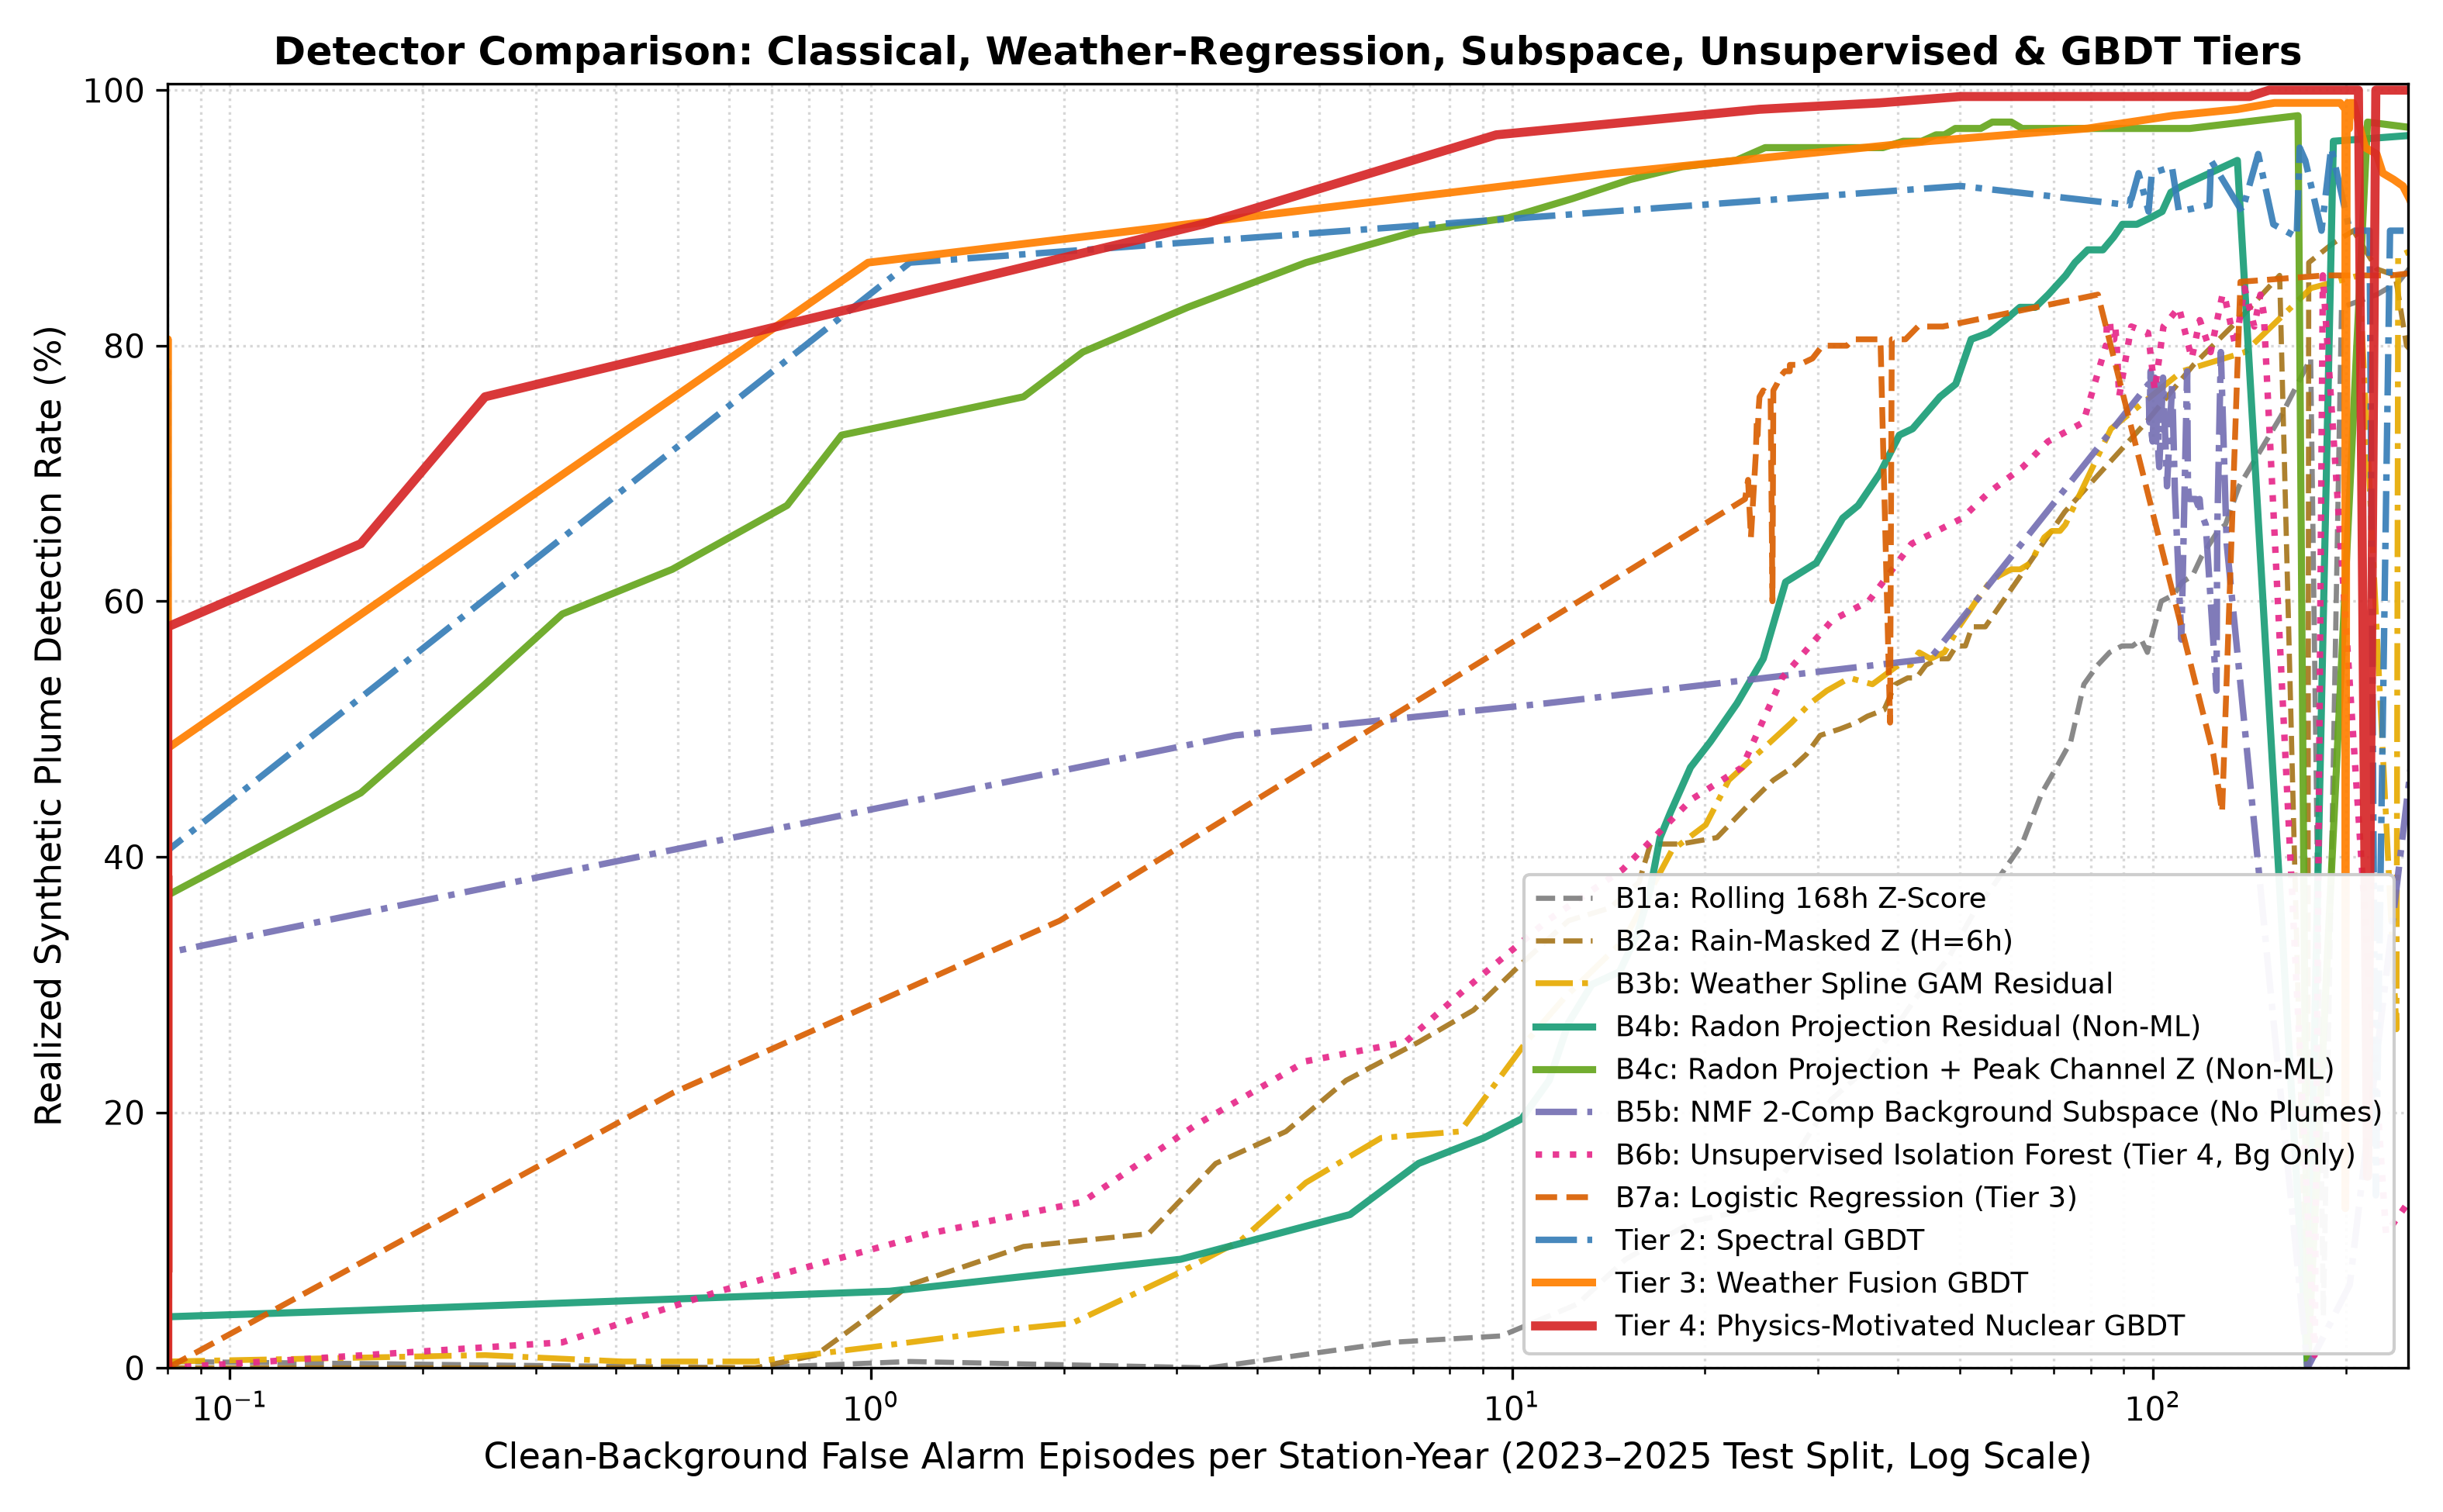
\includegraphics[width=0.86\textwidth]{reports/figures/rigorous_matched_roc_curves.png}
    \captionof{figure}{Receiver Operating Characteristic (ROC) matched detection curves comparing baseline rules against machine learning tiers on the test split.}
    \label{fig:roc_curves}
\end{center}

\vspace{0.6em}
\refstepcounter{subsection}
\addcontentsline{toc}{subsection}{3.8 The Rain-Masked Baseline Control Experiment}
\noindent\textbf{3.8 The Rain-Masked Baseline Control Experiment}\\[0.3em]
To rigorously answer whether complex machine learning is necessary or if a simple heuristic rule muting alarms during rainfall suffices, an explicit control experiment was developed (\url{src/evaluate_rain_masked_baseline.py}). The results at matched detection targets are summarized in Table~\ref{tab:control_experiment}.

\begin{center}
\captionof{table}{Rain-Masked Baseline Control Experiment at Matched Detection Targets}
\label{tab:control_experiment}
\small
\resizebox{\textwidth}{!}{%
\begin{tabular}{l c c c}
\toprule
\textbf{Baseline / Mask Rule} & \textbf{Lowest FA/yr at $\ge 87.12\%$ Det.} & \textbf{Lowest FA/yr at $\ge 91.88\%$ Det.} & \textbf{Max Det. (\%)} \\
\midrule
\textbf{Unmasked ($H = \text{none}$)} & 215.48 ($k=1.40$) & 303.03 ($k=0.75$) & 92.50\% \\
\textbf{Rain Mask: Rain only ($H = 0\text{h}$)} & 197.47 ($k=1.35$) & 285.77 ($k=0.75$) & 92.50\% \\
\textbf{Rain Mask: Rain + 3h ($H = 3\text{h}$)} & 179.80 ($k=1.30$) & 251.65 ($k=0.75$) & 92.50\% \\
\textbf{Rain Mask: Rain + 6h ($H = 6\text{h}$)} & 181.77 ($k=1.25$) & 245.98 ($k=0.75$) & 92.50\% \\
\textbf{Rain Mask: Rain + 12h ($H = 12\text{h}$)} & 177.49 ($k=1.25$) & 238.66 ($k=0.75$) & 92.00\% \\
\textbf{Tier 3 ML (Weather Fusion, Schema 2)} & $3.89$ & $3.89$ & $96.50\%$ \\
\textbf{Tier 4 ML (Nuclear Physics, Schema 3)} & $\mathbf{2.63}$ & $\mathbf{2.71}$ & $\mathbf{98.00\%}$ \\
\bottomrule
\end{tabular}%
}
\end{center}

The control experiment demonstrates that simply suppressing alarms during rain fails. To reach $\ge 91.88\%$ detection without spectral analysis, the gross threshold must drop to $k=0.75\sigma$, causing 238.66 false alarms/year from baseline noise. Tier 3 machine learning achieves a 97.6\% false alarm reduction over the best rain-mask heuristic, confirming the scientific necessity of multi-channel spectral and weather fusion.
\end{framed}

\newpage

% ==============================================================================
% BOX 10: REFERENCES
% ==============================================================================
\begin{framed}
\refstepcounter{section}
\addcontentsline{toc}{section}{REFERENCES}
\noindent\textbf{REFERENCES}\\[0.6em]
\noindent Abdelhakim, A., 2025. Anomaly detection in gamma-ray radiation spectra using artificial neural network and ant colony optimization. \textit{Journal of Environmental Radioactivity} 283, 107790. \url{https://doi.org/10.1016/j.jenvrad.2025.107790}\\[0.5em]
\noindent Alamaniotis, M., 2024. Mode-driven explainable artificial intelligence approach for estimating background radiation spectrum in a measurement applicable to nuclear security. \textit{Annals of Nuclear Energy} 209, 110849. \url{https://doi.org/10.1016/j.anucene.2024.110849}\\[0.5em]
\noindent Ayoub, A., Wainwright, H.M., Sansavini, G., 2024. Machine learning-enabled weather forecasting for real-time radioactive transport and contamination prediction. \textit{Progress in Nuclear Energy} 172, 105255. \url{https://doi.org/10.1016/j.pnucene.2024.105255}\\[0.5em]
\noindent Ayoub, A., Wainwright, H.M., Wang, L., Sansavini, G., 2024. An enhanced Fourier neural operator surrogate for radioactive plume transport forecasting. \textit{Stochastic Environmental Research and Risk Assessment} 38(8), 3173--3189. \url{https://doi.org/10.1007/s00477-024-02738-8}\\[0.5em]
\noindent Bandstra, M.S., Curtis, J.C., Ghawaly, J.M., Joshi, T.H., Bilton, K.J., 2023. Explaining machine-learning models for gamma-ray detection and identification. \textit{PLOS ONE} 18(6), e0286829. \url{https://doi.org/10.1371/journal.pone.0286829}\\[0.5em]
\noindent Bilton, K.J., Joshi, T.H., Bandstra, M.S., Curtis, J.C., Quiter, B.J., Cooper, R.J., Vetter, K., 2019. Non-negative matrix factorization of gamma-ray spectra for background modeling, detection, and source identification. \textit{IEEE Transactions on Nuclear Science} 66(5), 827--837. \url{https://doi.org/10.1109/TNS.2019.2907267}\\[0.5em]
\noindent Breitkreutz, H., Mayr, J., Bleher, M., Seifert, S., Stöhlker, U., 2023. Identification and quantification of anomalies in environmental gamma dose rate time series using artificial intelligence. \textit{Journal of Environmental Radioactivity} 259--260, 107082. \url{https://doi.org/10.1016/j.jenvrad.2022.107082}\\[0.5em]
\noindent Buckton, C.J., Wyngaardt, S.M., Ngxande, M., 2025. Radioisotope compositional analysis using Monte Carlo $\gamma$-ray simulations and regression neural network. \textit{Applied Radiation and Isotopes} 220, 111746. \url{https://doi.org/10.1016/j.apradiso.2025.111746}\\[0.5em]
\noindent Burnett, J.L., Croudace, I.W., Warwick, P.E., 2010. Short-lived variations in the background gamma-radiation dose. \textit{Journal of Radiological Protection} 30(3), 525--533. \url{https://doi.org/10.1088/0952-4746/30/3/007}\\[0.5em]
\noindent Cetnar, J., 2006. General solution of Bateman equations for nuclear transmutations. \textit{Annals of Nuclear Energy} 33(7), 640--645. \url{https://doi.org/10.1016/j.anucene.2006.02.004}\\[0.5em]
\noindent Currie, L.A., 1968. Limits for qualitative detection and quantitative determination. Application to radiochemistry. \textit{Analytical Chemistry} 40(3), 586--593. \url{https://doi.org/10.1021/ac60259a007}\\[0.5em]
\noindent Detwiler, R.S., Pfund, D.M., Myjak, M.J., Kulisek, J.A., Seifert, C.E., 2015. Spectral anomaly methods for aerial detection using KUT nuisance rejection. \textit{Nuclear Instruments and Methods in Physics Research Section A} 784, 339--345. \url{https://doi.org/10.1016/j.nima.2015.01.040}\\[0.5em]
\noindent Fjeldsted, A., Morrow, T., Scott, C., Hagen, A., 2024. A novel methodology for gamma-ray spectra dataset procurement over varying standoff distances and source activities. \textit{Nuclear Instruments and Methods in Physics Research Section A} 1064, 169681. \url{https://doi.org/10.1016/j.nima.2024.169681}\\[0.5em]
\noindent Frankemölle, J.P.K.W., Camps, J., De Meutter, P., Meyers, J., 2025. A Bayesian method for predicting background radiation at environmental monitoring stations in local-scale networks. \textit{Geoscientific Model Development} 18(6), 1989--2003. \url{https://doi.org/10.5194/gmd-18-1989-2025}\\[0.5em]
\noindent Hsieh, T.C., Li, C.H., Li, S.H., 2026. A minute-level analysis between environmental gamma dose rate and precipitation. \textit{IEEE Access} 13, 3649414. \url{https://doi.org/10.1109/ACCESS.2025.3649414}\\[0.5em]
\noindent ICRP, 1996. Conversion Coefficients for Use in Radiological Protection against External Radiation (ICRP Publication 74). \textit{Annals of the ICRP} 26(3--4), 5--19. \url{https://doi.org/10.1016/S0146-6453(96)90003-2}\\[0.5em]
\noindent Karafasoulis, K., Kyriakis, A., 2026. Anomaly detection in gamma-ray spectra using autoencoders with small form factor CZT detectors. \textit{Applied Radiation and Isotopes} 230, 112409. \url{https://doi.org/10.1016/j.apradiso.2025.112409}\\[0.5em]
\noindent Ke, G., Meng, Q., Finley, T., Wang, T., Chen, W., Ma, W., Ye, Q., Liu, T.Y., 2017. LightGBM: A highly efficient gradient boosting decision tree. \textit{Advances in Neural Information Processing Systems (NeurIPS 2017)} 30, 3146--3154. \url{https://proceedings.neurips.cc/paper_files/paper/2017/file/6449f44a102fde848669bdd9eb6b76fa-Paper.pdf}\\[0.5em]
\noindent Knoll, G.F., 2010. Radiation Detection and Measurement, fourth ed.. \textit{John Wiley \& Sons, Hoboken, NJ}. \url{https://www.wiley.com/en-us/Radiation+Detection+and+Measurement%2C+4th+Edition-p-9780470131480}\\[0.5em]
\noindent Lalor, P., Adams, H., Hagen, A., 2026. Sim-to-real supervised domain adaptation for radioisotope identification. \textit{Nuclear Instruments and Methods in Physics Research Section A} 1083, 171159. \url{https://doi.org/10.1016/j.nima.2025.171159}\\[0.5em]
\noindent Lye, A., Ong, Z.Y., Xiao, N., Patelli, E., 2025. Physics-enhanced machine learning for probabilistic risk assessment in nuclear safety: An overview, recent developments, and perspectives. \textit{Annals of Nuclear Energy} 218, 111562. \url{https://doi.org/10.1016/j.anucene.2025.111562}\\[0.5em]
\noindent Masson, O., Baeza, A., Bieringer, J., Brudecki, K., et al., 2011. Tracking of airborne radionuclides from the damaged Fukushima Dai-Ichi nuclear reactors by European networks. \textit{Environmental Science \& Technology} 45(18), 7670--7677. \url{https://doi.org/10.1021/es2017158}\\[0.5em]
\noindent Melintescu, A., Chambers, S.D., Crawford, J., Williams, A.G., Zorila, B., Galeriu, D., 2018. Radon-222 related influence on ambient gamma dose. \textit{Journal of Environmental Radioactivity} 189, 67--78. \url{https://doi.org/10.1016/j.jenvrad.2018.03.012}\\[0.5em]
\noindent Meng, L.J., Ramsden, D., 2000. An inter-comparison of three spectral-deconvolution algorithms for gamma-ray spectroscopy. \textit{IEEE Transactions on Nuclear Science} 47(4), 1329--1336. \url{https://doi.org/10.1109/23.872973}\\[0.5em]
\noindent Mercier, J.F., Tracy, B.L., d'Amours, R., Chagnon, F., Hoffman, I., Ungar, R.K., Korpach, E.P., 2009. Increased environmental gamma-ray dose rate during precipitation: a strong correlation with contributing air mass. \textit{Journal of Environmental Radioactivity} 100(7), 527--533. \url{https://doi.org/10.1016/j.jenvrad.2009.03.002}\\[0.5em]
\noindent Minato, S., 1980. Analysis of time variations in natural background gamma radiation flux density. \textit{Journal of Nuclear Science and Technology} 17(6), 461--469. \url{https://doi.org/10.1080/18811248.1980.9732610}\\[0.5em]
\noindent Moszyński, M., Nassalski, A., Syntfeld-Każuch, A., Szczęśniak, T., Czarnacki, W., Wolski, D., Pausch, G., Stein, J., 2006. Temperature dependences of LaBr$_3$(Ce), LaCl$_3$(Ce) and NaI(Tl) scintillators. \textit{Nuclear Instruments and Methods in Physics Research Section A} 568(2), 739--751. \url{https://doi.org/10.1016/j.nima.2006.06.039}\\[0.5em]
\noindent Paatero, J., 2000. Wet deposition of radon-222 progeny in northern Finland measured with an automatic precipitation gamma analyser. \textit{Radiation Protection Dosimetry} 87(4), 273--280. \url{https://doi.org/10.1093/oxfordjournals.rpd.a033008}\\[0.5em]
\noindent Sangiorgi, M., Hernández-Ceballos, M.A., Jackson, K., Cinelli, G., Bogucarskis, K., De Felice, L., Patrascu, A., De Cort, M., 2020. The European Radiological Data Exchange Platform (EURDEP): 25 years of monitoring data exchange. \textit{Earth System Science Data} 12(1), 109--118. \url{https://doi.org/10.5194/essd-12-109-2020}\\[0.5em]
\noindent Smith, A., Lott, N., Vose, R., 2011. The Integrated Surface Database: Recent developments and partnerships. \textit{Bulletin of the American Meteorological Society} 92(6), 704--708. \url{https://doi.org/10.1175/2011BAMS3015.1}\\[0.5em]
\noindent Sportisse, B., 2007. A review of parameterizations for modelling dry deposition and scavenging of radionuclides. \textit{Atmospheric Environment} 41(13), 2683--2698. \url{https://doi.org/10.1016/j.atmosenv.2006.11.057}\\[0.5em]
\noindent Stohl, A., Seibert, P., Wotawa, G., Arnold, D., Burkhart, J.F., Eckhardt, S., Tapia, C., Vargas, A., Yasunari, T.J., 2012. Xenon-133 and caesium-137 releases into the atmosphere from the Fukushima Dai-ichi nuclear power plant: determination of the source term, atmospheric dispersion, and deposition. \textit{Atmospheric Chemistry and Physics} 12(5), 2313--2343. \url{https://doi.org/10.5194/acp-12-2313-2012}\\[0.5em]
\noindent Sun, J., Niu, D., Liang, J., Li, L., 2024. Rapid nuclide identification algorithm based on self-attention mechanism neural network. \textit{Annals of Nuclear Energy} 207, 110708. \url{https://doi.org/10.1016/j.anucene.2024.110708}\\[0.5em]
\noindent Takeuchi, N., Katase, A., 1982. Rainout-washout model for variation of environmental gamma-ray intensity by precipitation. \textit{Journal of Nuclear Science and Technology} 19(5), 393--409. \url{https://doi.org/10.1080/18811248.1982.9734160}\\[0.5em]
\noindent Wen, S., Zhou, R., 2024. Temperature peak-drift correction method for NaI(Tl) detectors using the background peak. \textit{Sensors} 24(8), 2621. \url{https://doi.org/10.3390/s24082621}\\[0.5em]
\end{framed}

\end{document}
